\chapter{Results}\label{Sec:Results}

This chapter presents the results of the two positive-unlabeled learning approaches for maximal representative subsampling. The proposed PU learning techniques have been implemented slightly adjusted, while the idea to improve the assessment of classifiers in a non-traditional setting was preserved. The traditional ROC curve , with logistic regression and support vector machines. The discussions begin with the difficulties of working and dealing with data from two different sources.

\section{Decision-Trees for Data Processing}

Since errors and inaccuracies slipped in quickly, preparing the data took a particularly long time. To ensure that the data has been read and mapped accordingly, various decision-trees have been trained right from the start to detect for mismatch. In fact, this is already an application of the discriminative learning procedure.

\begin{figure}[ht]
\centering
\vspace{0.25cm}
   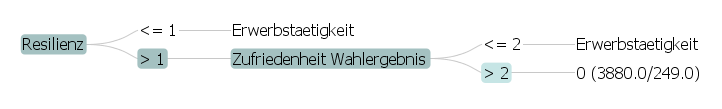
\includegraphics[scale=0.65,angle=0]{fig/treepath}
\captionsetup{width= 380pt}
\caption{Trees were trained using either sci-kit learn or WEKA explorer to identify preprocessing mistakes. The outer right path of the decision-tree demonstrates the desired behavior of the constructed model. "Resilienz"  and "Zufriedenheit Wahlergebnis" have been used to classify the majority of instances as GESIS. Both attributes have been measured on the same scale or mapped properly. Technically, this means that there was no better way to split the data at that specific node. Either the algorithm did not see any gain in continuing to split or the tree was fully grown first and then pruned back using out-of sample estimations.}
\end{figure}

Figure 4.1 visualizes a path of the latest J48 tree on the current set of features. The entire tree can be seen in the project repository. For the reasons mentioned in Chapter 2, tree-based algorithms are particularly suitable for quickly capturing incorrectly handled data. A subgroup of all participants is said to be representative of the target population, regarding the particular complexity of the trained model. Model complexity, with respect to the right-most leaf node, gives high confidence to include the subgroup of 249 GBS instances in the MRS. 

\vspace{0.33cm}
\begin{table}[ht]
    \begin{center}
		\captionsetup{width= 430pt}
            {\footnotesize
            \begin{tabular}{l|cccccccccc}
                \hline \hline
                           &  TP Rate & FP Rate & Precision & Recall & F-Measure & ROC Area & PRC Area & Class \\
                \hline
                      LMT & 0.971 & 0.655 & 0.916 & 0.971 & 0.943 & 0.878 & 0.979 & GESIS\\
                      & 0.345 & 0.029 & 0.619 & 0.345 & 0.443 & 0.878 & 0.519 & GBS\\
                \hline \hline
    		 J48 & 0.973 & 0.710 & 0.910 & 0.973 & 0.940 & 0.716 & 0.928 & GESIS\\
                      & 0.290 & 0.027 & 0.596 & 0.290 & 0.390 & 0.716 & 0.389 & GBS\\
\end{tabular}}
        \caption{J48 and LMT tree evaluation. These trees served as indicators for invalid mappings during development. The true negative rates of 0.029 and 0.027 indicate that there is just a small fraction of non-representative GBS instances. The constructed models are characterized by a high bias and low variance. Note that training was not an attempt to estimate the fraction of positives.}
\end{center}
\end{table}

\section{Maximal Representative Subsample}

The initial idea was to train a one-class classifier (OCC) by learning from training data containing only GESIS instances. This technique is very similar to PU learning. To identify survey participants amongst all GBS instances, representative sampling of the negative class is not strictly required \cite{tax}. In one-class SVM, the support vector model infered the properties of representative cases and from these properties predicted which GBS participants are unlike the representative examples. Predictions from the One-Class SVM are uncalibrated scores that have not been normalized and therefore can not be compared to models based on different algorithms. Instead, multiple OCCs have been trained on different  bootstrap samples from GESIS. The predicted probability was then derived by a majority decision. Figure 4.2 shows the fraction of correctly classified instances by the OCCs as a function of the parameter \(\nu\) on a hold-out set.

\begin{figure}[ht]
\centering
   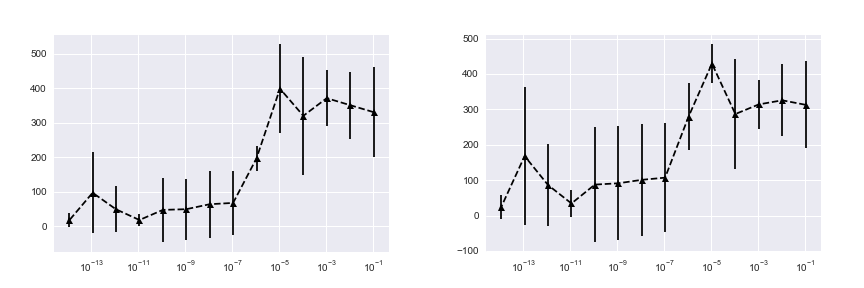
\includegraphics[scale=0.38,angle=0]{fig/occfigure}
\captionsetup{width= 380pt}
\caption{Tuning parameter \(\nu\) that controls the trade-off between the fraction of non-representative samples and the number of support vectors in one-class SVM. More than 0.73 of GBS (right) are classified as representative with low confidence (high sdt.) for the optimal value \( \nu = 10^5\). The plot on the left shows that not all GESIS participants have been classified as such.} 
\end{figure}

The OCC suffered from unavoidable variance in the learning task due to insufficient data points in the minority class GBS (n=579). There was clearly not enough data available to partition it into separate training and test sets without losing significant modelling or testing capability. The results of the ensemble were insufficient and unreliable. The question arises whether learning is feasible at all. To address this problem, less complex algorithms have been used in the PU training procedure (Algorithm 1). In model selection, logistic regression slightly outperformed linear SVMs with respect to the AUROC as can be seen in Figure 4.3. The optimized model then predicted the probability of every single instance in the combined dataset. The optimal threshold for the ROC curve with AUROC 0.62 gives an MRS consisting of a little less than half of the participants (\(\frac{271}{579}\)).

\begin{figure}[ht]
\centering
   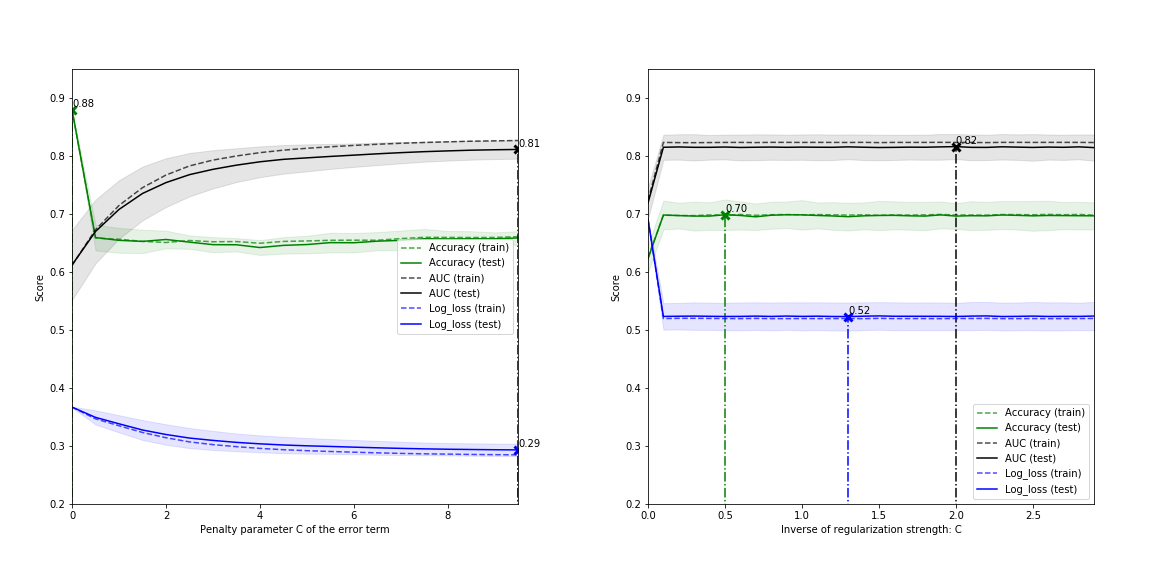
\includegraphics[scale=0.38,angle=0]{fig/gridfigure}
\captionsetup{width= 400pt}
\caption{GridSearchCV: Gridsearch using repeated 10-fold stratified cross-validation on \(\frac{1}{2}\) of the data to evaluate multiple scorers simultaneously. The baselines are 0.89 for accuracy, 0.82 for AUC/AUROC and 0.29 for logarithmic loss. The baselines outperform the trained models on the given metrics, due to the high imbalance in the data. Logistic regression (right) was slightly outperformed by Support Vector Machines (right).}
   \label{fig:Ng1} 
\end{figure}

The result set of Algorithm 1 could have remained unchanged for further studies. However, it is the case that the AUROC of 0.62 has not been adapted the for positive-unlabeled setting as described in Section 3. This is lies in the fact that no class prior of GBS was available. Subsequent runs have now been able to make use of the estimated fraction of latent positives. Instead of removing multiple misclassified instances, the implemented procedure trains classifiers iteratively to remove one instance at a time. This conceptually more intuitive when it comes to reducing sampling bias and seems less prone to overfitting. Fig. 4.4 demonstrates this procedure by plotting a ROC curve for the predicted probabilities of each classifier. The MRS is basically initialized with GBS itself and then subsampled step by step. Although this algorithm looks promising, further research must follow before it can be considered for MRS. 

\begin{figure}[ht]
\centering
   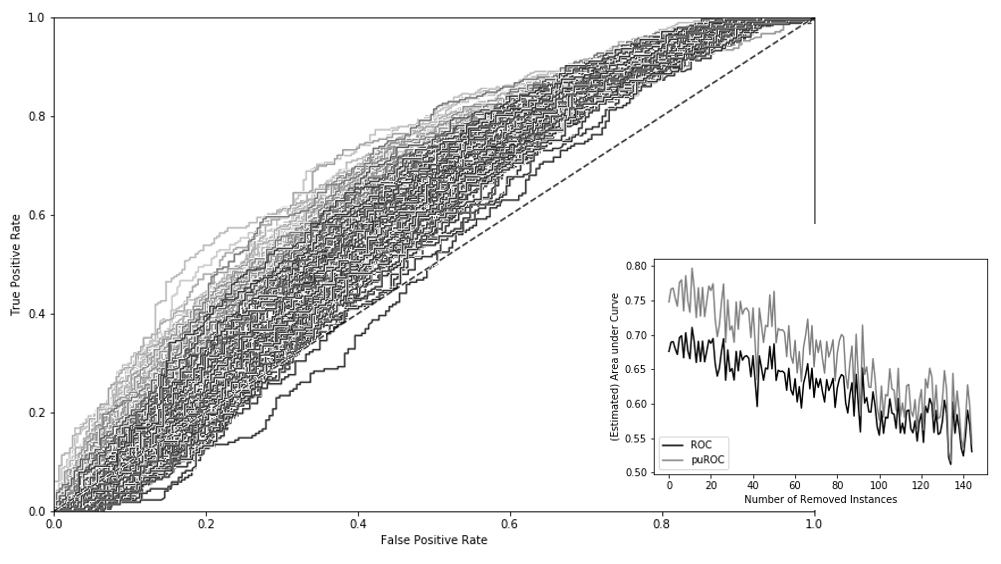
\includegraphics[scale=0.46,angle=0]{fig/res}
\captionsetup{width= 380pt}
\caption{ROC and puROC evaluation for PU learning with Random Forests as base models \cite{breiman2}. An AUROC of approximately \(\frac{1}{2}\) implies that there is no more evidence for covariate shift. Iterations stopped at an estimated decrease of \(\frac{1}{5}\). The remaining instances are considered representative of the target population.}
   \label{fig:Ng1} 
\end{figure}
